\chapter{Controlling Legged Locomotion}
\label{sec:ControllingLeggedLocomotion}
\index{control}

There are many different elements of legged locomotion control. This chapter covers two of the more well-known control algorithms: the first being a control algorithm based on the hopping robot from previous chapters, the second is a popular algorithm used by many robots in existence called the zero-moment-point method. The latter typically makes heavy use of motors placed at the joints that are being controlled to keep the center of mass of the robot in a desirable location, where the former uses a more dynamic placement-based method that keeps the robot's trajectory on a desired path.

%\section{Central Pattern Generator} % (notes page 67)
%\label{sec:CentralPatternGenerator}
%
%Central Pattern Generator: CPG. A collection of nerves that fire in sequence, generating "fictive locomotion" with no feedback from muscles. If the CPG were the whole story, locomotion would be feedforward. In reality, there is definitely feedback to the CPG.
%
%[ALAN] NEEDS MORE. Could be a very interesting section about the cat experiments from McMahon... I will have to hunt down that book somewhere here...

\section{Raibert Hopping Robot} %(notes page 34-39)
\label{sec:RaibertHoppingRobot}
\index{Raibert Robot}

Given the SLIP model of locomotion discussed in section \ref{sec:SLIP}, we want to know how we can control such a model. 

$I_{body}<<ml_{0}^{2}$: can't control $\theta_{c}$ in stance.
$I_{leg}<<I_{body}$: can control $\theta_{c}$ in flight.

Now let's assume compression in the spring is elastic: $E_{tot}$ = constant. The only control is $\theta_{c}$ at first contact. There are multiple approaches to control:

\subsection*{First Approach} Find a period solution. Given $l_{0}$, $k$, $m$, and $g$, find a $\theta_{c}^{*}$, $\dot{x}^{*}$, and $h^{*}$, at the apex of the hopper's flight, that will cause a motion that returns the hopper to the same conditions. Figure \ref{fig:SLIPPeriodicMotion} shows how we can find these initial conditions. By assuming symmetry about the apex of the motion, we can start the center of mass at its lowest point, with the spring compressed, and release it at a chosen velocity. If we then measure the angle at which the leg departs the ground, the height the center of mass reaches at the apex, and the forward velocity of the center of mass at the apex, we can use these quantities as our initial $\theta_{c}^{*}$, $\dot{x}^{*}$, and $h^{*}$.

% FIGURE
\begin{figure}[h]		% h="here" t="top" b="bottom" p="separate page"
\begin{centering}
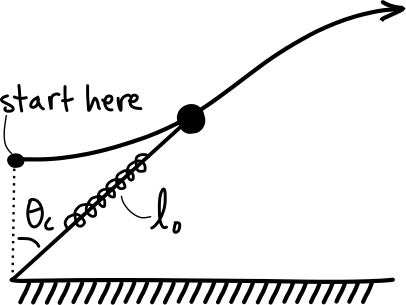
\includegraphics[width=0.4\textwidth]{Figures/SLIPPeriodicMotion}\par
\end{centering}
\caption[Diagram: SLIP Initial Conditions for Periodic Control]{SLIP initial conditions for periodic control. This diagram explains how to find initial conditions for the periodic method of SLIP control. If the motion is symmetric about the apex of the motion path, the initial conditions at the apex can be found by launching the mass from its lowest position at a chosen velocity.}
\label{fig:SLIPPeriodicMotion}
\end{figure}
%

However, this method of using periodic motion to control the locomotion of the hopper will likely be unstable. Nothing about this method of control indicates that the hopper will be able to reject disturbances in its gait. Previously, in section \ref{sec:SpringLoadedInvertedPendulum}, we briefly discussed using a linear controller to control the speed of the hopper: 

\begin{equation}
\theta_{c}=\theta_{c}^{*}+k(\dot{x}-\dot{x}^{*})+k_{2}(h-h^{*})
\label{eq:LinearController}
\end{equation}

In equation \ref{eq:LinearController}, the $k_{2}(h-h^{*})$ term is redundant because of energy conservation. 

***ASIDE ON EIGENVALUES was here in the notes. Page 36. Is it needed? I don't think it flows.***

\subsection*{Second Approach}

Insight and intuition. Raibert's way. Assume that energy is fixed. Observe that contact time, $T$, is almost independent of $\theta_{c}$. One can imagine that the hopper is simply a spring and a mass, fixed to the ground as shown in figure \ref{fig:SLIPCorrection}. The part of the trajectory of this spring-mass system that we care about is the lower half, which is analogous to the hopper's motion when the leg is touching the ground. This part of the motion of the hopper is assumed to be the same as this half-sine curve, with some correction made for the effect of gravity. 

% FIGURE
\begin{figure}[h]		% h="here" t="top" b="bottom" p="separate page"
\begin{centering}
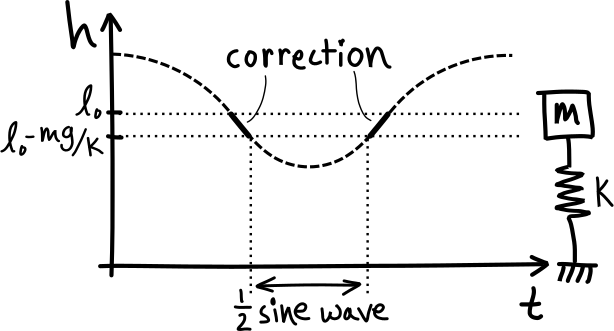
\includegraphics[width=0.6\textwidth]{Figures/SLIPCorrection}\par
\end{centering}
\caption[Diagram: SLIP Height Correction for Raibert Control]{SLIP height correction for Raibert control. Height of the hopper is plotted in time through the stance phase of the SLIP motion, which is marked between the corrections. For Raibert control, the motion of the hopper in the stance phase is equivalent to that of a simple vertically oscillating mass-spring system. This results in a sinusoidal hopper height as a function of time with a correction for the constant acceleration due to gravity.}
\label{fig:SLIPCorrection}
\end{figure}
%

The sine curve can be described as

\begin{equation}
y=y_{0}+A\sin{\left(t\sqrt{k/m}\right)}
\label{eq:SineCurve}
\end{equation}

Since we only care about the bottom half of the sine curve, we can surmise the following:

\begin{equation}
T\sqrt{k/m}=\pi
\label{eq:SineArgument}
\end{equation}

But we must also consider the correction:

\begin{equation}
T=\pi\sqrt{m/k}+\mbox{correction}
\label{eq:ContactTime}
\end{equation}

Note here that $T$ is not the period of the sine curve, but the contact time of the leg on the ground. The period of the hypothetical sine curve of the hopper's motion would be $2T$.

Then, we observe that steady motions are symmetric in the stance phase of the total trajectory. This is shown in figure \ref{fig:SLIPSymmetry}. 

% FIGURE
\begin{figure}[h]		% h="here" t="top" b="bottom" p="separate page"
\begin{centering}
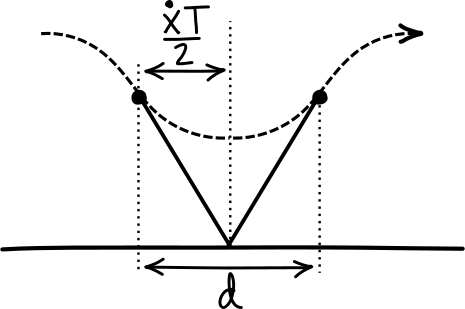
\includegraphics[width=0.45\textwidth]{Figures/SLIPSymmetry}\par
\end{centering}
\caption[Diagram: SLIP Symmetrical Stance Phase for Raibert Control]{SLIP symmetrical stance phase for Raibert controll. Since in the stance phase the height of the hopper is a sinusoidal function of time, the motion path is symmetrical. If the horizontal speed of the hopper is approximately constant, the width of the stance phase is $d = \dot{x}T$. This symmetry also allows for the painless calculation of $\theta_{c}$ requied to enforce this symmetry.}
\label{fig:SLIPSymmetry}
\end{figure}
%

Based on this assumption, we can derive a function that gives $\theta_{c}$ as a function of the horizontal speed of the center of mass of the hopper. To get that relationship, we first assume that the horizontal speed $\dot{x}$ is approximately constant throughout the entire gait cycle. This makes the calculation for $d$ trivial, $d=\dot{x}T$. From geometry then, we observe:

\begin{equation}
l_{0}\sin{\theta_{c}}=\frac{\dot{x}T}{2}
\label{eq:SLIPDistance}
\end{equation}

Since we are interested in $\theta_{c}$ as a function of $\dot{x}$, we solve equation \ref{eq:SLIPDistance} for $\theta_{c}$:

\begin{equation}
\theta_{c}=\arcsin{\left(\frac{\dot{x}T}{2l_{0}}\right)}
\label{eq:SLIPContactAngleBalance}
\end{equation}

Where $T$, the contact time, is found in equation \ref{eq:ContactTime}.

This derivation of $\theta_{c}$ is based entirely in the stance phase of the gait cycle, meaning all we have done is find a $\theta_{c}$ in terms of $\dot{x}$ that will keep the stance phase symmetric. Therefore we can think of this as a balance controller: given an initial forward velocity, the hopper will continue to go at that velocity, relatively unaffected by the balance controller's choice for $\theta_{c}$. To consider the linear speed controller that we found before, we simply add it to the balance controller:

\begin{equation}
\theta_{c}=\arcsin{\left(\frac{\dot{x}T}{2l_{0}}\right)}+k\left(\dot{x}-\dot{x}_{d}\right)
\label{eq:HopperController}
\end{equation}

K in this case must be small. This approach is similar to the first approach, but where the first has two free parameters, this tells us how to assign one of those parameters, $\theta_{c}$.

The second level of control: regulating energy level. First approach: measure E and add to it: $\mbox{energy}=k(E_{desired}-E)$. Second approach, Raibert style: dissipation per hop is monotonic in height. The dissipation per hop does not depend on the height of the hop. 

The third level of control: body orientation. Figure \ref{fig:SLIPBodyControl} shows the forces on a hopping robot's body that can be applied by motors. We can apply a moment on the leg during stance:

\begin{equation}
M=-k\theta_{b}-c\dot{\theta}_{c}
\label{eq:HopperBodyControl}
\end{equation}

% FIGURE
\begin{figure}[h]		% h="here" t="top" b="bottom" p="separate page"
\begin{centering}
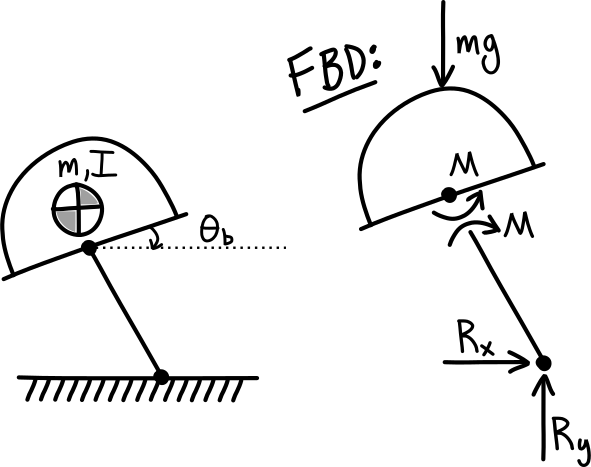
\includegraphics[width=0.5\textwidth]{Figures/SLIPBodyControl}\par
\end{centering}
\caption[Diagram: SLIP Free Body Diagram for Control]{SLIP free body diagram for Control. A free body diagram for the SLIP model was presented in section \ref{sec:SLIP}. This free body diagram also includes a moment $M$ acting at the hinge which is used for leg angle control.}
\label{fig:SLIPBodyControl}
\end{figure}
%

Assume all three controls are effectively decoupled. Each applies a very small amount of noise to the other. 

Going back to the first approach: root finding to get a periodic solution. What if we didn't care about the hopper returning to its initial conditions on the first bounce, but rather we wished it to return to the initial conditions after two bounces? We can solve numerically for this, and we call it a ``period two'' solution. Figure \ref{fig:SLIPPeriodic} shows the trajectory of the state-space map. Period two solutions in legged locomotion are typically seen as a ``limp.'' 

Text from the notes that I don't really know how to make sense of: `` Or you could look at the period one solutions, at what happens when you do one perturbation, and you get an eigenvalue of neg. 1, then in 2 steps, you get back to where you were. ''

% FIGURE
\begin{figure}[h]		% h="here" t="top" b="bottom" p="separate page"
\begin{centering}
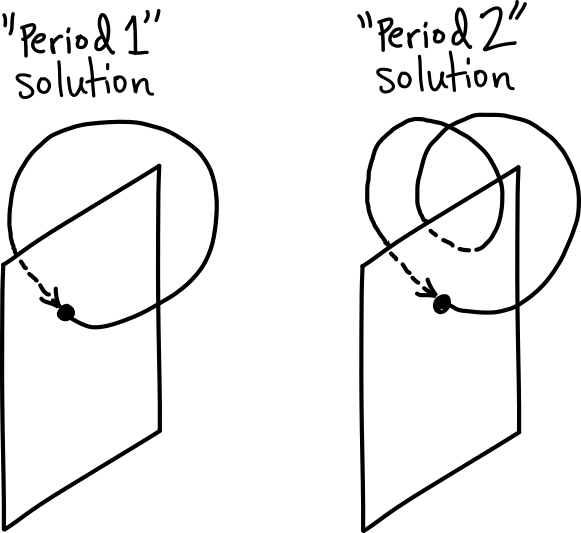
\includegraphics[width=0.4\textwidth]{Figures/SLIPPeriodic}\par
\end{centering}
\caption[Diagram: SLIP Periodicity and Limping]{SLIP periodicity and limping. The planes are phase-space planes. To the left is a description of typical systems, in which a operates at a single fixed point, and the system has the same state at the same point in any two periods. To the right is a description of a system operating in period 2, in which the state of the system alternates between two solutions at the end of each period. In the context of locomotion, this latter case is typically a model for limping gaits.}
\label{fig:SLIPPeriodic}
\end{figure}
%

\section{ZMP and Capture Point Method} %(notes page 60-64)
\label{sec:ZMPAndCapturePointMethod}
\index{ZMP}
\index{capture point method}

One popular method used to control modern legged robots is the zero-moment-point (ZMP) method. Honda's Asimo robot is a good example of a robot whose gait dominated by this method of control. Before getting into the details of this method of control, it is important to understand the basic result of using the ZMP method. Imagine a bipedal walking robot that uses the ZMP method of control. At any point in its gait, freeze the robot and lock all of its joints. Neglecting the momentum of the limbs, if the robot were frozen at any point in its gait, it would be able to stand. Each frozen frame of the robot's gait is a statically stable position because there is no \textit{net moment} on the robot's body. 

The method of control requires careful control of the joint angles. It also requires that the feet have some surface area that makes complete contact with the ground. In other words, the feet of the robot must be completely flat to make use of the torques produced at the joints. 

The basic program for operation of a robot that uses ZMP control starts with specifying all the joint angles of the robot as a function of time. This means that almost everything about the state of the system and its centers of mass is known. The velocities, joint forces, acceleration, torques, etc. can all be calculated. To calculate the forces in the system, an open kinematic chain can be used. Start with an open limb, like a hand, and do the free body diagram and momentum balances for it. Once the forces acting on the hand are calculated, the forces on the connecting limbs can also be calculated. 

%%
%% Vukabrotovic 1968,2004.
%%

The two-dimensional feet shown in figure \ref{fig:ZMPFoot} are statically equivalent. Since the ground only pushes upwards on the foot, all realizable force distributions have a ZMP inside the foot. The figure shows where the name ``Zero Moment Point" comes from; the ZMP is the point on the foot where the net force vector can be moved such that no net moment is exerted on the foot. 

% FIGURE
\begin{figure}[h]		% h="here" t="top" b="bottom" p="separate page"
\begin{centering}
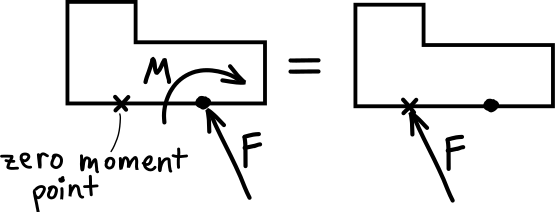
\includegraphics[width=0.5\textwidth]{Figures/ZMPFoot}\par
\end{centering}
\caption[Diagram: Zero Moment Point at Foot]{Zero moment point control at foot. An equivalent force system exists such that only a resultant force exists, and acts a so-called zero moment point. The location of the ZMP is determined by selecting a value for $\theta_{i}(t)$.}
\label{fig:ZMPFoot}
\end{figure}
%

One way of programming a robot to walk with a stable motion that uses this concept is to start with a specified joint angle control scheme in time, $\theta_{i}(t)$ and calculate the resulting ZMP at the foot. Then, check that the ZMP is always inside the outline of the foot. If the ZMP is not inside the foot, try different joint angle control scheme $\theta_{i}(t)$. However, this control strategy is incomplete. To find a working $\theta_{i}(t)$, the process needs to be repeated until a working $\theta_{i}(t)$ appears, which could take considerable time. It is helpful to know \textit{how} to change $\theta_{i}(t)$ such that we get a control scheme where the ZMP is always inside the foot. 

Consider a person standing in one place, as in figure \ref{fig:ZMPPerson}. In this diagram, C is the zero moment point. D is the desired location of the zero moment point. G is the point on the foot which is directly below the person's center of gravity. To stand still, G must equal C.

% FIGURE
\begin{figure}[h]		% h="here" t="top" b="bottom" p="separate page"
\begin{centering}
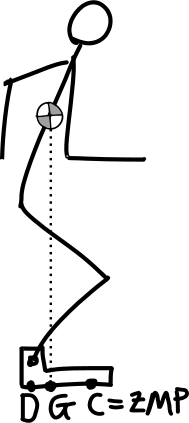
\includegraphics[width=0.2\textwidth]{Figures/ZMPPerson}\par
\end{centering}
\caption[Diagram: Zero Moment Point Control for Humans]{Zero moment point control for humans. The point $C$ is the ZMP, the point $G$ is located at the horizontal position of the center of mass, and the point $D$ is a desired location of the ZMP for control purposes. When $C$ and $G$ are at the same point, the human can stand still.}
\label{fig:ZMPPerson}
\end{figure}
%

Taking an angular momentum balance with respect to C, the average system rotation is in the direction of C to G. For example, the sum of the moments with respect to C is in the counter-clockwise direction. If $\vHdot_{/G'}$ is negligible, G accelerates away from C:

\begin{equation}
\vHdot_{/C}=\vr_{G'/C}\times\va_{G'}m+\vHdot_{/G'}
\label{eq:ZMPAMB}
\end{equation}

So an appropriate balance scheme is the following: place C so that G is between C and D, and G moves towards D as a result. Given that there is a force at the ankle, the ankle torque directly controls the location of C. This is a similar control scenario as the torque control of an inverted pendulum. 

%%
%% Perhaps expand upon the inverted pendulum stuff...
%%

Now consider a person walking. A similar ZMP control strategy to the one applied to standing can also be used for walking. The first step in a ZMP walking control strategy is to generate a trajectory of the robot and all the joints such that the ZMP is always inside the convex hull of the feet. The convex hull of the feet is illustrated by figure \ref{fig:ConvexHull}; it is the region of minimum perimeter that includes the outlines of both feet. When there is only one foot on the ground, the convex hull of the feet is the same as the outline of one foot. 

% FIGURE
\begin{figure}[h]		% h="here" t="top" b="bottom" p="separate page"
\begin{centering}
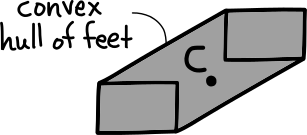
\includegraphics[width=0.3\textwidth]{Figures/ConvexHull}\par
\end{centering}
\caption[Diagram: Convex Hull of Feet]{Convex hull of feet. This diagram shows both feet in a top down view, and both feet are contacting the ground. The shaded area is the convex hull of the feet, which is the minimum-perimiter closed linear spline that includes both feet. If only one foot is on the ground, then the convex hull is the outline of only that one foot. For ZMP control, the zero moment point must be within the convex hull at all times.}
\label{fig:ConvexHull}
\end{figure}
%

The next step in a ZMP walking control strategy is to apply it to a robot and correct errors if the measured C does not equal D. There are three ways to correct for such errors. The first is corralling like for standing; however, this strategy doesn't work if G is outside of the convex hull. The second way to get C to equal D is to quickly bend the body to move the center of mass and exert a force at the feet. The third way is to adjust a step the robot was going to take anyway. The robot should take a bigger step if falling unintentionally forwards, and smaller if falling backwards. This is where the concept of capture regions comes from. A capture region is a set of places that a robot can put its foot and then find a control strategy that will allow it to end up standing still, given that the robot is already falling from one foot to the other.

%%
%% Cite Jerry Pratt for something in here. 
%% I had also wanted to mention something about stilts in here. 
%%

